%% AMS-LaTeX Created with the Wolfram Language : www.wolfram.com

\documentclass{article}
\usepackage{amsmath, amssymb, graphics, setspace}

\newcommand{\mathsym}[1]{{}}
\newcommand{\unicode}[1]{{}}

\begin{document}

\title{Inequalities}
\author{}
\date{}
\maketitle



In 1 and 2, let \textit{ a} and \textit{ b} be positive real numbers 

Prove that \(\sqrt{a b}\leq \frac{a+b}{2}\) { }with equality if and only if \(a=b\).

How does \(\frac{2}{\frac{1}{a}+\frac{1}{b}}\) compare with the two quantities in the first problem? Hint: Consider the lengths \(\overline{\text{AM}}\),
\(\overline{\text{GM}}\), and \(\overline{\text{GH}}\).

\begin{doublespace}
\noindent\(\pmb{\text{Import}[\text{{``}/Users/kennethlevasseur/Desktop/Screen Shot 2014-09-24 at 10.40.56 AM.png{''}}]}\)
\end{doublespace}

\begin{doublespace}
\noindent\(\)
\end{doublespace}



\pmb{ The AM/GM inequality }generalizes $\#$1: { } If all \(a_i\) are non-negative real numbers, then



$\quad \quad \quad $\(\left(a_1a_2\cdots  a_n\right){}^{1/n}\leq  \frac{a_1+a_2+\cdots +a_n}{n}\)



with equality if and only if all the \(a_i\) are equal.

An express delivery service restricts the size of packages it will accept. { }Packages cannot exceed 18 inches in length plus girth, i. e., \(\text{length}+2\times
\text{width} +2\times \text{height}\leq 18\). { }Find the maximum volume of an acceptable package.

 Let \(a_1, a_2. \ldots  , a_{n }\) be positive, with sum 1. { } { }Show that \(\sum _{i=1}^n a_i^2\geq \frac{1}{n}\) { }and { } \(\sum _{i=1}^n
a_i^4\geq \frac{1}{n^3}\)

(a) { }Compute the determinant \(D= \left\left| \left(
\begin{array}{ccc}
 a & b & c \\
 c & a & b \\
 b & c & a \\
\end{array}
\right)\right\right|\) two ways to derive the identity \(a^3+b^3+c^3-3 a b c =(a+b+c) \left(a^2+b^2+c^2-a b-b c - c a\right)\).



(b) { }Prove that if \(x\), \(y\), and \(z\) are distinct real numbers, then \(\sqrt[3]{x-y}+ \sqrt[3]{y-z}+\sqrt[3]{z-x}\neq 0\).

Let \(x_1+x_2+x_3=\frac{\pi }{2}\), where the \(x_i\) are positive. { } Show that { }\(\sin  x_1\sin  x_2 \sin  x_3\leq \frac{1}{8}\).

Let \(f\)be a continuous and monotonically increasing function such that \(f(0) = 0\) and \(f(1) = 1\). Prove that { } \\
 { } { } { } { }\(f(0.1)+f(0.2)+\cdot  \cdot  \cdot +f(0.9)+f^{-1}(0.1)+f^{-1}(0.2)+\cdot  \cdot  \cdot +f^{-1}(0.9) \leq  9.9\)

Let \(T\) be a tetrahedron with three mutually perpendicular edges of lengths \(a\), \(b\), and \(c\). { }Let \(l\) be the sum of the length of the
six edges of \(T\). { }What is the maximum possible volume of \(T\)?

Let \(a_1, a_2, \ldots  , a_n\) be positive real numbers and let \(s\) be their sum. { }Show that 



\(\left(1+a_1\right)\left(1+a_2\right)\cdots \left(1+a_n\right) \leq  1 + \frac{s}{1!}+ \frac{s^2}{2!}+ \cdots +\frac{s^n}{n!}\).$\quad $

For positive numbers \(x\) and \(y\), prove that \(x^x+y^y\geq x^y+ y^x\), with equality if and only if \(x=y\).



over for more



\pmb{ Definition}: A function \(f\) defined on an interval $\mathcal{I}$ (possibly infinite) is \textit{ concave} if for all \(a, b\in \mathcal{I}\)
and \(\lambda \in (0,1)\), \(\lambda  f(a) + (1-\lambda )f(b)\leq f(\lambda  a+(1-\lambda )b)\).



\textit{ Quick question}: { } How does concavity relate to the second derivatives of functions that are twice differentiable?



\pmb{ Jensen{'}s inequality:} { }If \(f\) is a concave function, and \(\lambda _1, \lambda _2, \ldots , \lambda _n\) are positive real numbers that
add to 1, { }then \(\sum _{i=1}^n \lambda _if\left(a_i\right)\leq f\left(\sum _{i=1}^n \lambda _ia_i\right)\).

What does Jensen's inequality say if \(\lambda _i= \frac{1}{n}\), and { }\(f(x) = \ln  x\), and how does it relate to the AM/GM inequality?







The Cauchy-Schwarz (AKA Cauchy$--$Bunyakovsky$--$Schwarz, or CBS) inequality has both discrete and continuous versions. { }The real discrete version
is that if \(x\) and \(y\) are vectors in \(\mathbb{R}^n\), then { }\(\left(\sum _{i=1}^n x_i y_i\right){}^2\leq \left(\sum _{i=1}^n x_i^2\right)\left(
\sum _{i=1}^n y_i^2\right)\), with equality if and only if the two vectors are scalar multiples of one another. { } This comic gives the continuous
version:

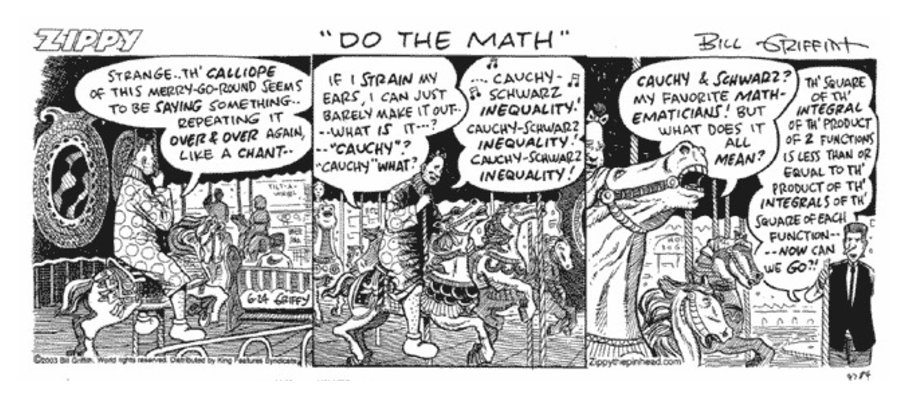
\includegraphics{92.420_inequalities_2018_gr1.eps}

Find the maximum of the function \(f(x,y,z)=5x -6y+7z\) on the ellipsoid \(2x^2+3y^2+4z^2=1\).


\subsection{Assignment due on Oct 31}


\item A solution/attempt for your second problem.


\item A solution/attempt at one of the problems numbered 10, 11, or 12.

\end{document}
